\section{Search With Clojure}
\label{sec:search-with-clojure}
	Clojure's excellent \gls{jvm} interoperability permits the use of countless third-party libraries.  The most extensively used was Lucene.
	
	\subsection{Full-Text Search Using Lucene}
		\textcquote{luc-home}{Apache Lucene\texttrademark\ is a high-performance, full-featured text search engine library written entirely in Java.}  Lucene implements the document model, and provides a simple yet powerful and feature-rich \gls{api} to perform full-text search.  Among these features is the ability to vectorize documents according to the vector space model, utilize the extended document model to provide search of semi-structured documents, and issue search queries against the index.
	
	\subsection{Indexing Relational Database}
		The indexing of relational objects is a complicated process.  The objects must be retrieved from the relational database, transformed into documents from named tuples, then placed in the index.  Additionally, all foreign keys (\cref{def:foreign-keys}) must be encoded as documents (\cref{sec:encoding-entity-group-as-document-group}) in order to satisfy \cref{sec:mapping-entity-groups-to-documents}.
		
		The schema graph (\cref{def:schema-graph}) must be defined before the relational database may be crawled.
		
		\subsubsection{Schema Graph Definition}
		\label{sec:entity-schema}
			The schema graph is defined using a list.  Each schema component, whether an entity or entity group, is defined by \texttt{EntitySchema} records.  Each record accepts a map which specifies how each class of document should be indexed and identified.  The keys of this map are given in \cref{tbl:entity-schema-keys}.
			
			\begin{table}
				\centering
				
				\begin{tabular}{lp{9cm}l}
					\toprule
					Key & Description & Type(s) \\
					\midrule
					\texttt{:T} & Entity (\texttt{:entity}) or entity group (\texttt{:entity}) & Symbol \\
					\texttt{:C} & Table name for entities, brief description for entity groups & Symbol or String \\
					\texttt{:sql} & \Gls{sql} query used to construct the entity or entity schema & Expression \\
					\texttt{:ID} & Attribute or attributes that comprise the key (\cref{def:keys}) & Symbol or list of symbols \\
					\texttt{:attrs} & List of attributes to analyze to fields & List of symbols \\
					\texttt{:values} & List of attributes to index as values, must be subset of \texttt{:attrs} & List of symbols \\
					\bottomrule
				\end{tabular}
				
				\caption{Keys expected by \texttt{EntitySchema} records}
				\label{tbl:entity-schema-keys}
			\end{table}
		
		\subsubsection{Crawling the Relational Database}
			With the schema graph defined, the system is able to crawl the relational database, yielding a sequence of named tuples.  It iterates through every \texttt{EntitySchema} record, instructing every record to crawl itself given a database connection and index writer (\cref{clj:building-the-index}).
			
			\begin{figure}
				\begin{singlespaced}
					\begin{pygments}{clj}
(doseq [ent-def schemas]
  (crawl ent-def db-conn idx-w))
					\end{pygments}
				\end{singlespaced}
				
				\caption{Building the index}
				\label{clj:building-the-index}
			\end{figure}
			
			The \texttt{Database} protocol provides an \texttt{execute-query} method that permits access to the database.  In the current implementation, the \texttt{Sqlite3} record implements the \texttt{Database} protocol.  This record issues the query as-is, applying a given function to every result.
			
			Each record issues a \gls{sql} query against the database that retrieves all named tuples that it represents.  This query is given by the \texttt{:sql} key of the record.  For every symbol defined by the \texttt{:values} key, an additional query is issued.  These queries retrieve all distinct (within the context of that relation and attribute) values.
		
		\subsubsection{Transformation}
			For every named tuple, a document is constructed.  In addition to the attributes, several other fields may be added to the document.  These special fields contain additional meta information about the document.  For example, the class, type, and unique identifier are added to an entity, while an entity group has a space-delimited list of unique identifiers that comprise the group.
			
			Before becoming a document, named tuples are transformed into an internal representation.  The internal representation adds flexibility to the system; so long as functions exist to convert between the internal representation and other forms, the source of the data is irrelevant.
			
			Clojure permits the annotation of data with metadata.  Named tuples are returned as maps, with key-value pairs representing attributes and values for the tuple.  Metadata may be associated with a named tuple.  The metadata does not affect its key-value pairs.
			
			The map of attributes and values of a named tuple is annotated with the function \texttt{(with-meta obj map)}.  The \texttt{obj} parameter is the named tuple, while \texttt{map} is a map of metadata as defined by the system.  The keys of \texttt{map} for each type (value, entity, or entity group) are defined in \cref{tbl:type-metadata}.  The internal representation of the named tuple given in \cref{tbl:hmr-properties-rel} is given in \cref{clj:with-meta-internal-rep}.
			
			\begin{table}
				\begin{subtable}[b]{0.33\linewidth}
					\centering
					
					\begin{tabular}{ll}
						\toprule
						Key & Value \\
						\midrule
						:type & :value \\
						:class & <rel>|<attr> \\
						\bottomrule
					\end{tabular}
					
					\caption{Value}
				\end{subtable}
				\begin{subtable}[b]{0.33\linewidth}
					\centering
					
					\begin{tabular}{ll}
						\toprule
						Key & Value \\
						\midrule
						:type & :entity \\
						:class & <rel> \\
						:ID & <rel>|<pk> \\
						\bottomrule
					\end{tabular}
					
					\caption{Entity}
				\end{subtable}
				\begin{subtable}[b]{0.33\linewidth}
					\centering
					
					\begin{tabular}{ll}
						\toprule
						Key & Value \\
						\midrule
						:type & :group \\
						:entities & <rel>|<pk> \\
						 & [<rel>|<pk> \ldots] \\
						\bottomrule
					\end{tabular}
					
					\caption{Entity Group}
				\end{subtable}
				
				\caption{Metadata associated with each type}
				\label{tbl:type-metadata}
			\end{table}
			
			\begin{figure}
				\begin{singlespaced}
					\begin{pygments}{clj}
(with-meta
  {:code    "CDPS 101"
   :title   "Human-Mutant Relations"
   :subject "CDPS"}
  {:type  :entity
   :class :course
   :id    "course|cdps_101"})
					\end{pygments}
				\end{singlespaced}
				
				\caption{Internal representation of named tuple from \cref{tbl:hmr-properties-rel}}
				\label{clj:with-meta-internal-rep}
			\end{figure}
			
			Once the internal representation is constructed, it may be transformed into a document.  The mapping of a map to document is trivial; a field is created for every key in the map and the value corresponding to the key is the value of the field.  Unfortunately Lucene does not facilitate the storage of metadata.  Therefore the system must deal with metadata in a different way.
			
			The system modifies each key of the metadata; two underscores are prepended and appended to the key name.  This allows the system to differentiate between metadata and attributes.  The transformation from internal representation to document is given in \cref{tbl:internal-rep-to-document}.
			
			\begin{table}
				\centering
				
				\begin{tabular}{ll}
					\toprule
					Field & Value \\
					\midrule
					code & cdps 101 \\
					title & human mutant relations \\
					subject & cdps \\
					\_\_type\_\_ & entity \\
					\_\_class\_\_ & course \\
					\_\_id\_\_ & course|cdps\_101 \\
					\bottomrule
				\end{tabular}
				
				\caption{Document of internal representation from \cref{clj:with-meta-internal-rep}}
				\label{tbl:internal-rep-to-document}
			\end{table}
		
		\subsubsection{Indexing}
			With the named tuples transformed into documents, the index may be constructed.  The first step is to open the index for writing.  In Lucene, this is accomplished by creating an \texttt{IndexWriter} object on a \texttt{Directory} object that points to the index location.  The \texttt{IndexWriter} object also expects an analyzer to be used by default on documents it indexes.  The system uses a \texttt{WhitespaceAnalyzer} by default, but offers the ability to choose a different analyzer for specific fields.
			
			For every named tuple, the transformed document is written to the index by the index writer object.  In addition, the indexing document of every entity group is added.
		
	\subsection{Keyword Search in Document Space}
	\label{sec:keyword-search-document-space}
		With the entity graph encoded into the document model, users may begin issuing search queries.  Every query follows the following pattern:  users look up values (optionally using fuzzy search), these values are used to locate entities, and once two entities are selected, the system attempts to connect the two.
		
		\subsubsection{Fuzzy Value Search}
			Recall that entity values are stored as their \(n\)-gram (\cref{sec:n-gram}).  This allows users to make character substitutions, deletions, or additions, and still return values they may have intended on finding.  Without the use of \(n\)-grams, a misspelling on the user's part may result in an empty set of values being returned.  Values that are approximately matched would be assigned a lower score than those which are fully matched, but they would at least appear in the results.
			
			Rather than guessing the user's intention, the system presents the user with a list of values in order to give them the option of substituting their entry for an approximate match.  This autosuggest feature is intended to improve the user experience by eliminating a source of frustration -- irrelevant results as a result of a simple spelling error.
		
		\subsubsection{Flexible Keyword Search \gls{api}}
			The system provides a simple -- yet flexible -- keyword search \gls{api}.  Recall the extended query (\cref{ex:extended-query}) is in the form
			\[
				\query(\field, \w)
			\]
			
			The search \gls{api} provides a function that accepts a field to search in, as well one or more words to search for.  A phrase query comprised of every word is constructed.
			\[
				\query(\field, \w_1, \w_2, \dotsc, \w_n) = \bigcap_{\w \in \{\w_1, \w_2, \dotsc, \w_n\}} \query(\field, \w)
			\]
			
			Another function, \texttt{boolean-query}, accepts one or more \(\query\) functions as well as a boolean operator for each and returns the result.  The symbols \texttt{:and}, \texttt{:or}, and \texttt{:not} provide \(\cap\), \(\cup\), and \(\neg\), respectively.
			
			\begin{ex}[\texttt{boolean-query}]
				For example, the query in \cref{ex:extended-query} is given in \cref{clj:boolean-query}.
				
				\begin{figure}
					\begin{singlespaced}
						\begin{pygments}{clj}
(boolean-query
 [[:and (query :subject ``MATH'')]
  [:and (query :text ``class'')]])
						\end{pygments}
					\end{singlespaced}
					
					\caption{Boolean query in Clojure}
					\label{clj:boolean-query}
				\end{figure}
			\end{ex}

	\subsection{Graph Search in Document Space}
		With the ability for users to find relevant entities using fuzzy value search and the flexible keyword search \gls{api} (\cref{sec:keyword-search-document-space}), they must be able to find connections between two entities.  As previously stated, the document encoding of relational data is a graph.  This allows the system to search for links between entities by utilizing one or more graph search algorithms, such as \gls{bfs}.
		
		\subsubsection{A Case For Graph Search}
			Tuples are fragments, or facts, of larger pieces of knowledge.  By utilizing graph search, we amalgamate these facts to provide a user with a broader view.
			
				By utilizing graph search, we can take the facts in \cref{tbl:facts} and compose new facts.  For example, we could learn who teaches Complex Analysis.  It also allows us to ask questions, such as ``who taught Complex Analysis with Instructor X?''
			
			\begin{table}
				\begin{subtable}[b]{0.5\linewidth}
					\centering
					
					\begin{tabular}{ll}
						\toprule
						Field & Terms \\
						\midrule
						code & \(\{\text{math}, \text{360}\}\) \\
						title & \(\{\text{complex}, \text{analysis}\}\) \\
						subject & \(\{\text{math}\}\) \\
						\bottomrule
					\end{tabular}
					
					\caption{Fact representing a Course}
					\label{subtbl:fact-course}
				\end{subtable}
				\begin{subtable}[b]{0.5\linewidth}
					\centering
					
					\begin{tabular}{ll}
						\toprule
						Field & Terms \\
						\midrule
						id & \(\{\text{math}\}\) \\
						name & \(\{\text{mathematics}\}\) \\
						\bottomrule
					\end{tabular}
					
					\caption{Fact representing a Subject}
					\label{subtbl:fact-subject}
				\end{subtable}
				
				\caption{Fragments, or facts, of information in a dataset}
				\label{tbl:facts}
			\end{table}
			
			This automated discovery of relations between facts is why graph search is important.
		
		\subsubsection{Graph Search Algorithms}
			Recall we defined a graph as \(\sgraph{} = (\text{V}, \text{E})\), where \(\text{V}\) is the set of all facts in the database, and \(\text{E}(\egraph{})\) is the set of entities in entity group \(T\).  We say that two vertices in \(\egraph{}\) are connected if, and only if.
			\[
				\text{E}(\egraph{}) \cap \text{E}(\egraph{}') \not= \emptyset
			\]
			
			We must, given a keyword query \(\q\), find a subgraph, \(H\) of \(\sgraph{}\), such that
			
			\begin{itemize}
				\item The vertices, or hops, in \(H\) are minimized; and
				\item The satisfaction of keywords in \(\q\) by the vertices in \(H\) are maximized
			\end{itemize}
			
			In order to accomplish this, we find all vertices by entity group search and call this \(C\).  A graph search algorithm is used to minimally connect the vertices in \(C\).
			
			\begin{algorithm}[!ht]
				\caption{\(\textsc{Graph-Search}(C)\)}
				\label{alg:graph-search}
				
				\begin{singlespaced}
					\begin{algorithmic}[1]
						\REQUIRE \(C\) is a list of vertices
						\ENSURE minimal path between vertices in \(C\)
						\medskip
						\STATE \(s \in C\)
						
						\FOR{\(t \in C - \{s\}\)}
							\STATE find path connecting \(s \rightarrow t\) such that \(\textsc{Length}(\text{path}) \le \text{max-hops}\)
						\ENDFOR
						
						\RETURN path
						\medskip
						\medskip
					\end{algorithmic}
				\end{singlespaced}
			\end{algorithm}
		
		\subsubsection{Graph Search in Document Space}
			The question becomes:  why do we perform this graph search in document space?  Why not on the original relational space?  There are two main answers to this question:  speed and flexibility.
			
			Rather than relying on scanning every tuple in every relation in a relational database, the document model represents every tuple as a semi-structured document.  The contents of every field in these documents is indexed by an inverted list index data structure which permits fast lookup of documents based on keywords.  We utilize this property to quickly locate the initial ``source'' vertices.
			
			During the indexing process, various analyzers are applied against the text.  These may, for instance, remove the suffix of words; a process called stemming \cite{porter-97}.
			
			\begin{ex}[Porter Stemmer]
				A course may have ``mathematics'' or even ``mathematical'' in the title.  By utilizing a stemmer, we match both.  The Porter stemming algorithm returns ``mathemat'' as the root word for both of the examples.
			\end{ex}
			
			Other analyzers may remove stop words.  Stop words may include ``and'', ``or'', ``not'', etc.  These are functional words that may be removed from the text corpus without adversely affecting the meaning whose presence may otherwise affect the quality of search results \cite{silva-03}.
			
			Our implementation uses a document to represent edges in the entity graph.  By using the document model, we are able to quickly locate all other vertices connected to a specific vertex.
			
			\begin{ex}[Search for Connected Entities]
				Given the indexing documents \(x_1, x_2, x_3\)
				
				\begin{align*}
					x_1[\text{``entities''}] &= \{\text{course|math\_360}, \text{subject|math}\} \\
					x_2[\text{``entities''}] &= \{\text{course|math\_101}, \text{subject|math}\} \\
					x_3[\text{``entities''}] &= \{\text{course|cdps\_101}, \text{subject|cdps}\} \\
				\end{align*}
				
				A query, \(\q\) for entities in the subject ``math''.
				\[
					\q = \query(\text{``entities'', ``subject|math''}) \cap \query(\text{``\_\_type\_\_'', ``entity''})
				\]
				
				Would yield the results \(x_1, x_2\).
			\end{ex}
		
		\subsubsection{Breadth-First Search}
			\citeauthor*{cormen-09} define \gls{bfs} as follows
			
			\begin{displayquote}[\cite{cormen-09}]
				Given a graph \(G = (V, E)\) and a distinguished source vertex \(s\), breadth-first search systematically explores the edges of \(G\) to ``discover'' every vertex that is reachable from \(s\). It computes the distance (smallest number of edges) from \(s\) to each reachable vertex. It also produces a ``breadth-first tree'' with root \(s\) that contains all reachable vertices. For any vertex \(v\) reachable from \(s\), the path in the breadth-first tree from \(s\) to \(v\) corresponds to a ``shortest path'' from \(s\) to \(v\) in \(G\), that is, a path containing the smallest number of edges. The algorithm works on both directed and undirected graphs.
			\end{displayquote}
			
			Essentially \gls{bfs} populates the frontier before exploring the next hop.  Thus \gls{bfs} is able to explore a large, sparsely connected graph quickly.  However, if the graph is dense, \gls{bfs} would consume a substantial amount of memory, making an algorithm such as \gls{dfs} more suitable.
			
		\subsubsection{Functional \gls{bfs}}
			The simple nature of \gls{bfs} makes it ideal to implement in a functional manner.  There is minimal shared state or side effects, allowing the search to be conducted recursively.  Newly discovered vertices are conjoined with the existing queue to form a new queue.  Due to Clojure's persistent data structures, this operation is more efficient than intuition would dictate.
			
			The functional implementation of \gls{bfs} combines state changes into larger units.  This leaves large segments of the implementation free of side effects.  We exploit this fact to implement \gls{bfs} concurrently in Clojure.
		
		\subsubsection{Concurrent \gls{bfs}}
			In our implementation, the exploration of adjacent nodes is performed concurrently.  Rather than exploring each node sequentially, as show in \cref{fig:concurrent-initial}, \cref{fig:concurrent-sequential}, and finally \cref{fig:concurrent-concurrent}, nodes ``course|math\_101'' and ``course|math\_360'' are explored simultaneously.
			
			\begin{figure}
				\centering
				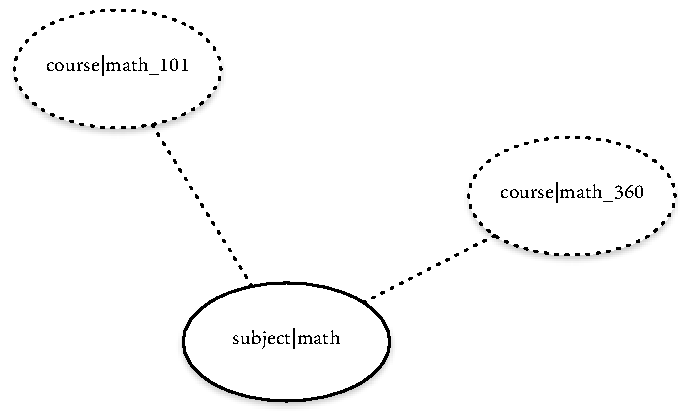
\includegraphics[scale=0.9]{figures/graphs/concurrent/initial}
				
				\caption{Initial graph}
				\label{fig:concurrent-initial}
			\end{figure}
			
			\begin{figure}
				\centering
				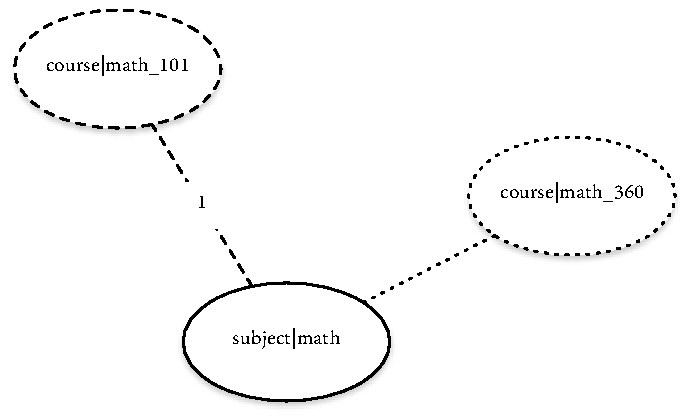
\includegraphics[scale=0.9]{figures/graphs/concurrent/sequential}
				
				\caption{Exploring the first adjacent node sequentially}
				\label{fig:concurrent-sequential}
			\end{figure}
			
			\begin{figure}
				\centering
				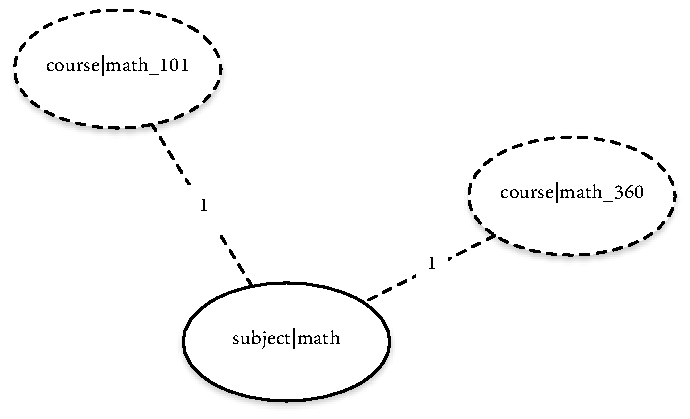
\includegraphics[scale=0.9]{figures/graphs/concurrent/concurrent}
				
				\caption{Both adjacent nodes explored}
				\label{fig:concurrent-concurrent}
			\end{figure}
		
		%
		%Distributed functional description of BFS
		%
		%Implementation details:
		%- Ref
		%- Atoms
		%- Agent
		%
		%\begin{itemize}
		%	\item Search in document graph using graph search algorithms with functional implementations: (Ford Fulkerson, BFS)
		%	\item Speed up using concurrency
		%	\item Clojure specific optimization: ref + atom
		%\end{itemize}